\chapter{Dataset}
\label{ch3}
Data preprocessing is an essential step in producing an effective machine learning model. The data for training must be representative of the problem being modeled, and the validation and test sets should be representative of the train dataset. Failing to satisfy these conditions can lead to an ineffective model, validation results that lead to poor model and hyperparameter selection, and testing results that inaccurately represent a model's capability. This Chapter steps through the preprocessing applied to the $C_{n}^{2}$ and weather data including filtering, window averaging, formatting into input sequences and forecasts, and parsing into train, validation, and test datasets.

\section{Measurement Collection Setup}

\subsection{Weather Measurements}
The entire dataset uses time correlated weather and $C_{n}^{2}$ measurements. The weather measurements are from a Davis Instruments Vantage Pro2 Plus weather station \cite{davis} deployed in front of an office building from 12 April 2020 through 10 August 2020. The weather variables recorded by the station and considered in this work are temperature, pressure, relative humidity, wind speed, and solar irradiance. Table \ref{tab:weather_station} lists the technical specs of the weather station including the measurement resolution, accuracy, and archive interval.
\begin{table}[h!]
	\begin{center}
		\caption{Davis Instruments Vantage Pro2 Plus Weather Station Measurements}
		\label{tab:weather_station}
		\begin{tabular}{||l|c|c|c||}
			\hline
			Variable & Resolution & Accuracy $\pm$ & Archive Interval \\
			\hline
			\hline
			Temperature & 0.1\textdegree C & 0.3\textdegree C & 1 min \\
			\hline
			Pressure & 0.1 mb & 1.0 mb & 1 min \\
			\hline
			Relative Humidity & 1\% & 2\% & 1 min \\
			\hline
			Wind Speed & 0.45 m/s & 5\% & 1 min \\
			\hline
			Solar Irradiance & 1 $W/m^{2}$ & 5\% & 1 min \\
			\hline
		\end{tabular}
	\end{center}
\end{table}

The variable resolution refers to the minimum difference measurable, for example relative humidity can distinguish between 90\% and 91\%, but not between 90\% and 90.5\%. The resolution of wind speed, 0.45 m/s, is 1 mph (mile per hour) resolution converted to m/s. Variable accuracy is the variable error per measurement, so for example a measurement of relative humidity of 90\% is has an error range of $\pm$ 2\%. Finally, the archive interval indicates how often the variable is reported. The archive interval is different from the measurement frequency. The anemometer measures wind speed every 2.5 to 3 seconds but the average over the archive interval, 1 minute, is reported. The archive interval of this dataset is 1 minute, the shortest interval available from the weather station.

The location of the weather station is on a storm drain surrounded by grass, about 20 feet to the southwest of a single-story office building. The weather station is not obscured by any trees or shrubbery in very close proximity. To the south of the weather station about 180\textdegree field of view is completely open space. The wind measurements are taken by an anemometer about 3 meters \ac{AGL}. The other measurements are recorded about 2.5 meters \ac{AGL}. Figure \ref{fig:setup_weather} illustrates the location of the weather station and labels the key sensors and solar panel. The image in Figure \ref{fig:setup_weather} is taken from the southeast to illustrate the proximity of the station to surrounding geography to the northwest. To the right of the image is the office building about 20 feet away.
\begin{figure}[h!]
	\centering
	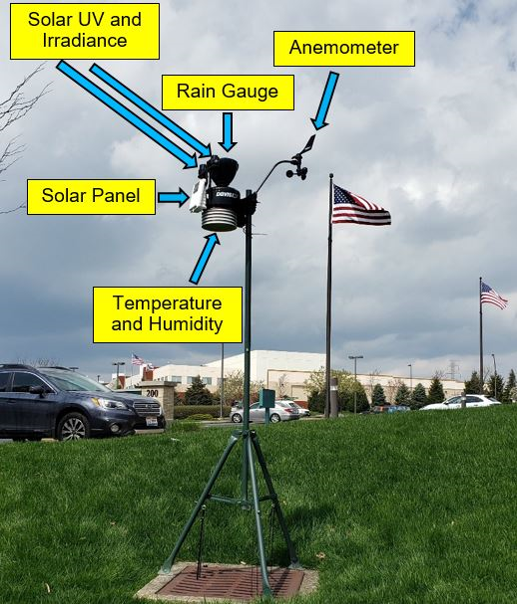
\includegraphics[width=0.65\textwidth]
	{setup_wx_station.png}
	\caption{Weather station deployment}
	\label{fig:setup_weather}
\end{figure}

\subsection{Turbulence ($C_{n}^{2}$) Measurements}
\label{sec:summary_tub_meas}
The other component of the dataset is minute-by-minute measurements of $C_{n}^{2}$ as measured by an MZA \ac{DELTA} turbulence profiler \cite{mzaassociatescorporation}. The \ac{DELTA} is a passive imaging sensor that uses a monochrome camera attached to a 6-inch telescope with 1.5 m focal length. The \ac{DELTA} calculates differential jitter as a function of angular separation to measure $C_{n}^{2}$ by collecting 300 frames (images) of a target of opportunity at 100 Hz. It's desirable for the target to have  high contrast features like edges and corners throughout the image to make measurements of differential jitter at variety of separations. Separations of 0.5 to 20 aperture diameters are recommended, so for a 6" telescope aperture the smallest feature separation would be 3" and largest 10' apart in the target plane.

The $C_{n}^{2}$ measurements in this work span from 12 April 2020 through 10 August 2020. During this time the \ac{DELTA} was deployed on the 5th floor of Fitz Hall at University of Dayton in Dayton, Ohio. Figure \ref{fig:setup_DELTA_a} is a picture of the \ac{DELTA}'s deployment in Fitz Hall.
\begin{figure}[p!]
	\centering
	\subfloat[Telescope setup\label{fig:setup_DELTA_a}]{
		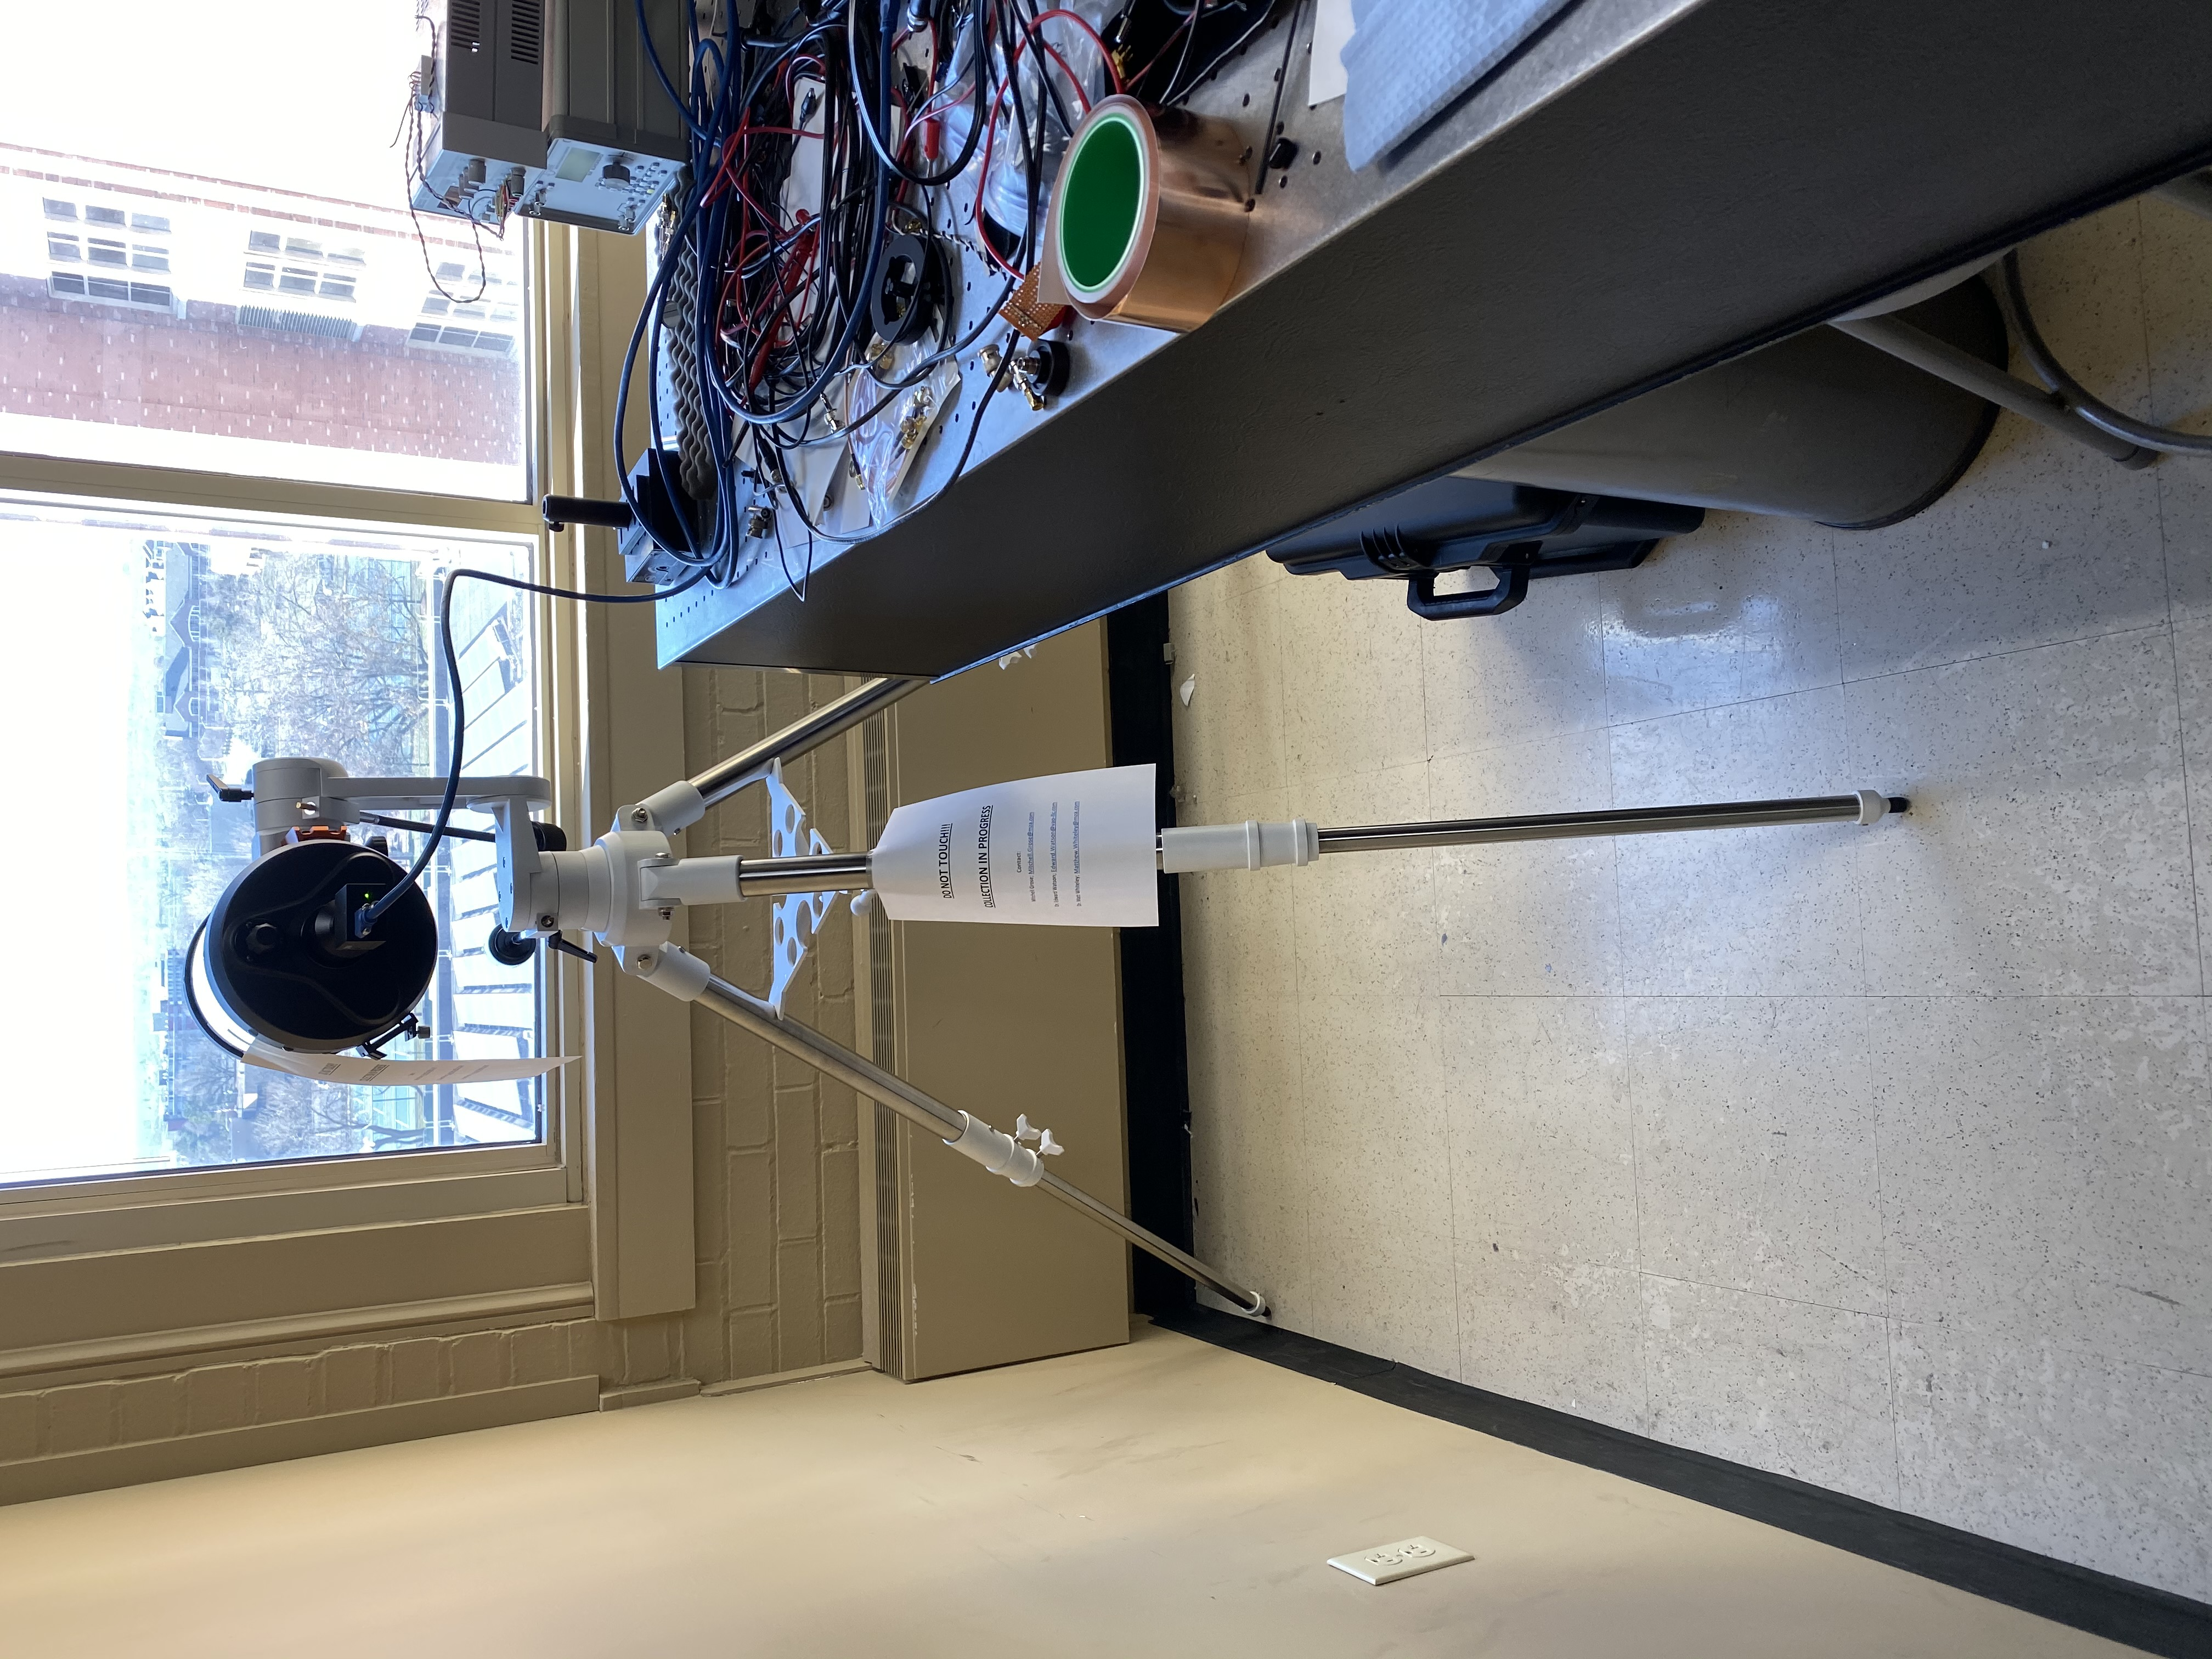
\includegraphics[width=0.49\textwidth]
		{DELTA_setup1.png}
	}
	\subfloat[Wide view of target\label{fig:setup_DELTA_b}]{
		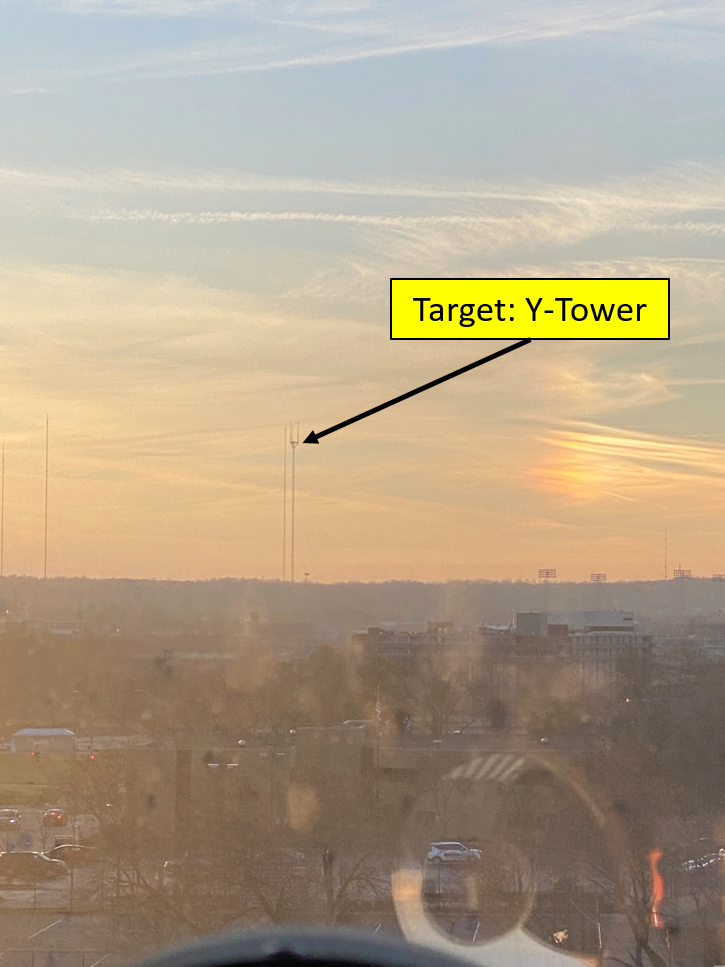
\includegraphics[width=0.49\textwidth]
		{DELTA_setup3.png}
	}
	\hfill
	\subfloat[Narrow view of the target\label{fig:setup_DELTA_c}]{
		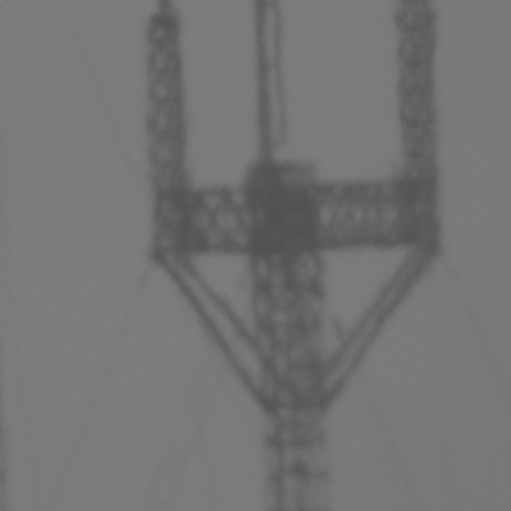
\includegraphics[width=0.49\textwidth]
		{Y_Tower.png}
	}
	\subfloat[Target as seen by the DELTA\label{fig:setup_DELTA_d}]{
		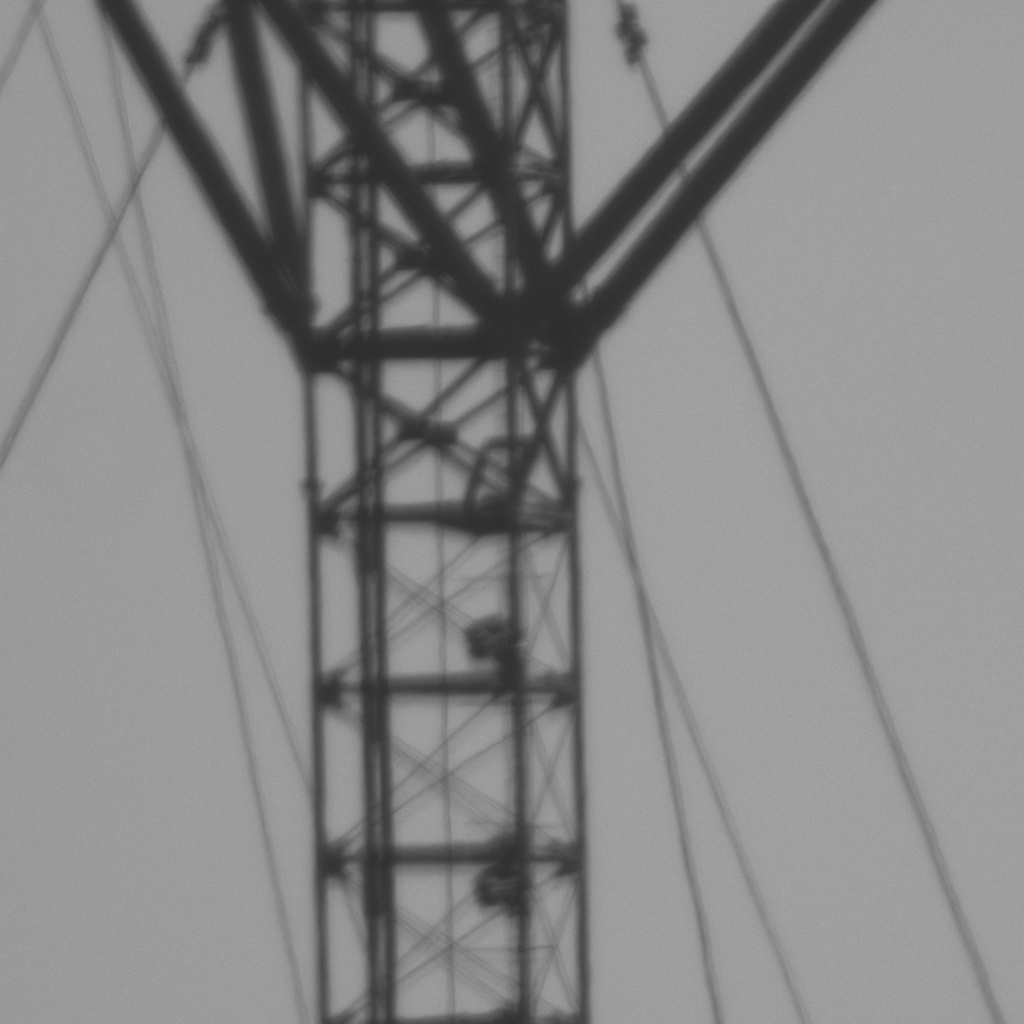
\includegraphics[width=0.49\textwidth]
		{FirstFrame_LowTurb.png}
	}
	\hfill
	\caption{DELTA setup for and target view for collection of minute-by-minute $C_{n}^{2}$ measurements.}
	\label{fig:setup_DELTA}
\end{figure}
The target the \ac{DELTA} observes throughout the collection is the \textit{WRGT/WKEF TV Dayton} tower to the southwest of the sensor. The range to the target is 6.4km. The platform is approximately 249 meters \ac{AMSL}, and the part of the target being imaged is estimated to be 566 meters \ac{AMSL}. Figure \ref{fig:setup_DELTA_b} illustrates a wide field-of-view (WFOV) picture of the target being imaged by the \ac{DELTA}. Figure \ref{fig:setup_DELTA_c} illustrates an narrow field-of-view (NFOV) image of the target during  turbulent conditions. Figure \ref{fig:setup_DELTA_d} is a single frame from a \ac{DELTA} image set during an evening neutral event (low $C_{n}^{2}$ strength). The sharp contrast in foreground and background and the abundance of edges and corners (features) make the target in Figure \ref{fig:setup_DELTA_d} excellent for the \ac{DELTA}. The tower target is dubbed the ``Y-Tower" because from the view of the \ac{DELTA} the target looks like a ``Y" as shown in Figures \ref{fig:setup_DELTA_c} and \ref{fig:setup_DELTA_d}.

As stated above, the \ac{DELTA} calculates differential jitter as a function of angular separation to measure $C_{n}^{2}$. It's the calculation of $C_{n}^{2}$ at 10 locations along the observation path that make the \ac{DELTA} a turbulence profiler in comparison with another sensor, like a Scintillometer, which reports only a single $C_{n}^{2}$ for the entire propagation path. The locations, or screens, of these $C_{n}^{2}$ measurements are at 5\%, 15\%, ..., 85\%, 95\% along the propagation path. In this work the profiling action is not utilized. Rather, the measurements along the path at each minute are uniform-path averaged for a single $C_{n}^{2}$ measurement per collection that is representative of the entire path. Although a uniform-path average is applied, the propagation path's geometry with respect to the terrain is highly relevant to the $C_{n}^{2}$ measurements at each screen and the \emph{type} of propagation path this work investigates.

Figure \ref{fig:DELTA_prop_geometry_a} illustrates the geometry of the propagation path. The y-axis is the path altitude \ac{AGL}, and the x-axis is the path range. Each blue bar represents a DELTA screen at the aforementioned normalized locations along the propagation path. The average screen altitude, 175m, is drawn as a magenta dashed line.
\begin{figure}[h!]
	\centering
	\subfloat[Path geometry\label{fig:DELTA_prop_geometry_a}]{
		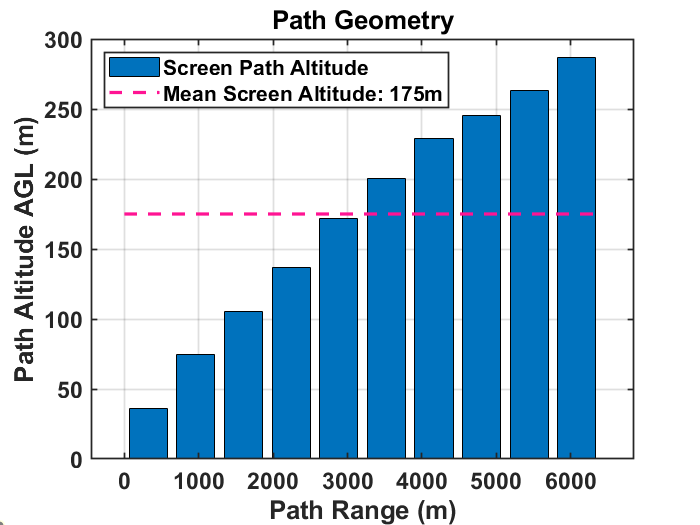
\includegraphics[width=0.49\textwidth]
		{path_geometry.png}
	}
	\subfloat[Terrain geometry\label{fig:DELTA_prop_geometry_b}]{
		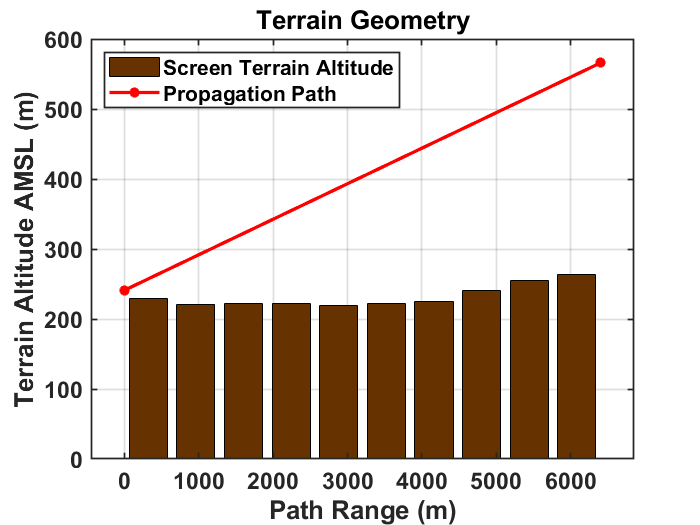
\includegraphics[width=0.49\textwidth]
		{terrain_geometry.png}
	}
	\hfill
	\caption{DELTA propagation path geometry}
	\label{fig:DELTA_prop_geometry}
\end{figure}
Similarly, Figure \ref{fig:DELTA_prop_geometry_b} illustrates with brown bars the altitude \ac{AMSL} of the terrain at the \ac{DELTA} screens. The propagation path is illustrated as the red line. Note that the angle of the propagation path with respect to the terrain bars in Figure \ref{fig:DELTA_prop_geometry_b} is misleading because the x-axis and y-axis limits on the plot are not scaled the same.

The \ac{DELTA} screens \ac{AGL} in Figure \ref{fig:DELTA_prop_geometry_a} illustrate that the altitude as a function of propagation path linearly increases for nearly the entire path. The average path altitude, 175m, is between the 5th and 6th screen. The height of the brown bars in Figure \ref{fig:DELTA_prop_geometry_b} illustrate that the altitude of the terrain as a function of the propagation path does not significantly change over the 6.4 km. This path illustrates that this work builds a machine learning model which forecasts $C_{n}^{2}$ at an average altitude of 175m AGL over 6.4 km. This geometry is unique as many long-term $C_{n}^{2}$ collections do not include these significant altitude changes and average altitude.

\subsection{Spatial Relationship of Platforms and Target}
The location of the \ac{DELTA} ($C_{n}^{2}$) platform is approximately 8.87 km to the west of the Vantage Pro2 Plus (weather) platform, and the Y-Tower being imaged by the DELTA is approximately 6.40 km to the southwest of the \ac{DELTA} platform. The combination of these paths puts the Vantage Pro2 Plus platform approximately 15.05 km from the Y-Tower. Figure \ref{fig:setup_geometry} illustrates the spatial relationship between the three locations of relevance, where each yellow circle marker are approximate locations.
\begin{figure}[h!]
	\centering
	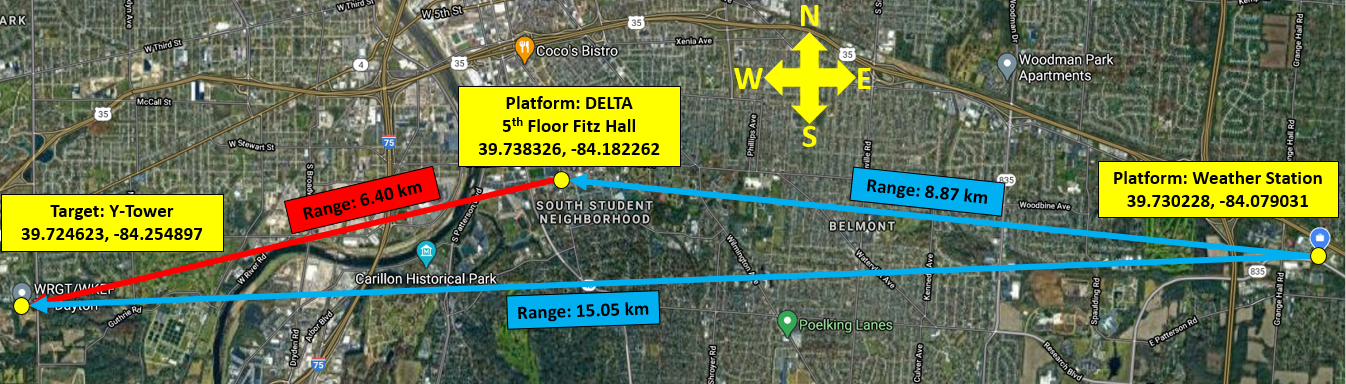
\includegraphics[width=0.99\textwidth]
	{setup_geometry.png}
	\hfill
	\caption{Spatial relationship between the DELTA platform, Vantage Pro2 Plus (weather) platform, and the Y-Tower (DELTA) target.}
	\label{fig:setup_geometry}
\end{figure}
Above each circle is a label of the location being marked and its latitude and longitude. The red arrow pointing from the \ac{DELTA} platform marker to the Y-Tower marker represents the \ac{DELTA} propagation path being processed to a $C_{n}^{2}$. The blue arrows point from the Vantage Pro2 Plus platform marker to the \ac{DELTA} platform marker and Y-Tower target marker.

Figure \ref{fig:setup_geometry} illustrates one of the significant challenges of this work. There is significant spatial separation of the $C_{n}^{2}$ path and weather measurements. Turbulence by nature is a highly variable process and adding a gap between 8.87 km and 15.05 km from the weather measurements to the $C_{n}^{2}$ path adds another layer of complexity. The weather measurements at the particular platform location may or may not be correlated with the $C_{n}^{2}$ measurements to the west, and the degree of correlation is vulnerable to change in time. For example, on a cloudless day, the solar irradiance trends are likely highly correlated with the $C_{n}^{2}$ trends, but on a day with scattered clouds the $C_{n}^{2}$ measured at a particular minute might be in the sunshine but the correlated solar irradiance measurement is in the clouds. This modeling effort is especially subject to the spatial separation since the experiment is performed in Ohio, a state known for high weather variability on a day-to-day and even hour-to-hour timescale. Data processing to focus on trends is meant in part to dampen the effect of high frequency events that are not well correlated between the $C_{n}^{2}$ path and weather measurements platform.

A theoretical advantage to modeling with the simple \ac{RNN}, \ac{GRU-RNN}, and \ac{LSTM-RNN} is to combat against the significant spatial separation of the weather measurements and $C_{n}^{2}$ path. Weather tends to flow from west to east, so from Figure \ref{fig:setup_geometry} the $C_{n}^{2}$ measurements will be impacted by weather that is measured at a later time at the weather platform. These architectures process the input sequences as a time-series, thus it's theorized the networks could capture relationships between the measured $C_{n}^{2}$ and weather conditions that are not temporally synced. 

\section{Data Preprocessing}
\subsection{Filtering, Window Averaging, and Interpolating}
\label{sec:filt_winavg_interp}
\subsubsection{Filtering}
The MZA \ac{DELTA} reports two metrics for each measurement: image confidence and $C_{n}^{2}$ confidence. The confidence levels each range from 0\% to 100\% and as the names suggest report the quality of the image sequence used for the calculation of $C_{n}^{2}$ and the quality in the $C_{n}^{2}$ calculation, i.e., the quality of the differential jitter measurements as a function of angular separation. The $C_{n}^{2}$ measurements can be easily quality-filtered by only keeping measurements which satisfy two user specified thresholds. In this work the thresholds are set to 50\% and 70\% minimum image and $C_{n}^{2}$ confidence, respectively. Figure \ref{fig:delta_confidences} illustrates the image and $C_{n}^{2}$ confidences of each measurement as a function of local time-of-day throughout the experiment as blue and orange markers, respectively.
\begin{figure}[h!]
	\centering
	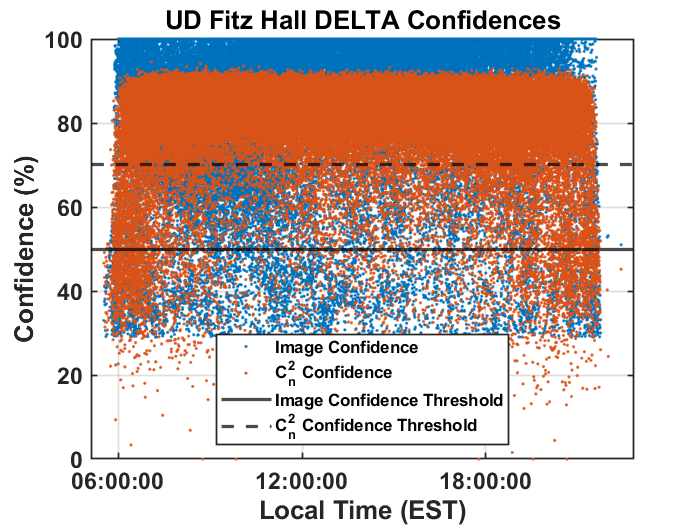
\includegraphics[width=0.7\textwidth]
	{DELTA_confidences.png}
	\hfill
	\caption{DELTA image and $C_{n}^{2}$ confidences.}
	\label{fig:delta_confidences}
\end{figure}
The black solid and dashed black lines represent the image and $C_{n}^{2}$ thresholds. A $C_{n}^{2}$ measurement is removed if an orange marker is below the dashed black line \emph{or} if a blue marker is below the solid black line. The majority of the $C_{n}^{2}$ confidences throughout the day are above the specified threshold. Most of the measurements removed due to $C_{n}^{2}$ confidences are in the early morning and late evening when target illumination is less than ideal resulting in poor differential jitter measurements. The image threshold filtering is more uniform across the entire day. A high $C_{n}^{2}$ confidence is more important to a measurement than a high image confidence, so the threshold for the image confidence is lower. Of the 76,186 measurements that passed the confidence thresholds, the average image and $C_{n}^{2}$ confidences are over 91\% and 83\%, respectively.

The Vantage Pro2 Plus weather station does not report data quality metrics on a per-variable basis. Evaluation of weather measurements in plots does not raise questions of data quality, both in the raw measurement value for a check of nonphysical values, and measurement trends for a check that the temporal rate of change of the measurements is realistic.

\subsubsection{Window Averaging}
After quality filtering, the weather and $C_{n}^{2}$ measurements are window averaged. A written returns an array of window averaged datetimes (dates + times) and corresponding window averaged measurements given four inputs. The four inputs are an input array of datetimes, an input array of measurements, a window width, and an interval size. The window width determines the temporal width the function uses to calculate an average. For example, given a window width of five minutes the window will look at $\pm$ 2.5 minutes around the current time being averaged. Any measurements $\ge$ to the current time minus 2.5 minutes and $<$ the current time plus 2.5 minutes is included in the average. The datetime returned for this example window averaged measurement is exactly the middle of the window. The interval size determines the temporal step each iteration. For example, given an interval size of one minute, the function will perform a window average about minute 07:05 on a given day, then step to perform a window average about minute 07:06. This iteration stops when the window includes a datetime beyond the last datetime in the array of measurements.

This modeling effort focuses on learning the relationship between the trends of prior environmental measurements and future $C_{n}^{2}$ measurements. To achieve this the window average uses a width of 30 minutes ($\pm$ 15 minutes) and interval of 1 minute. This wide window significantly smooths the weather and $C_{n}^{2}$ measurements to dampen high-frequency events and amplify the trends. This more significantly impacts the $C_{n}^{2}$ measurements which are highly stochastic by nature. 

\subsubsection{Interpolating}
After window averaging both sets of measurements, each is linearly interpolated to datetimes from 12 April 2020 through 10 August 2020 sampled every 30 minutes. The linear interpolation is performed by an open-source robust implementation from \textit{NumPy} \cite{harris2020array}. For each set of interpolations (weather and $C_{n}^{2}$), only interpolations less than 30 minutes are kept. Those that do not pass this condition are simply set to NaN (Not a Number) to preserve the arrays of measurements and datetimes sampled every 30 minutes. After this step the data is reduced to 5809 measurements at a 30 minute sample rate.

\subsection{Formatting into Sequences and Forecasts}
\subsubsection{Nighttime $C_{n}^{2}$ as Input Sequences}
A limitation of the experimental setup described in Section \ref{sec:summary_tub_meas} is the passive imager DELTA lacking an illuminated target. As a result, $C_{n}^{2}$ measurements before 06:00 and after 22:00 are entirely absent. Without a method to fill the nighttime $C_{n}^{2}$ this modeling technique is unable to incorporate prior $C_{n}^{2}$ measurements as an input variable to the model. It's hypothesized that including prior $C_{n}^{2}$ as an input will improve modeling performance as it will provide the model information about the trend of $C_{n}^{2}$ leading up to the forecast. The model is expected to learn that it's first forecast timestamp should follow the leading trend. If results indicate the inclusion of prior $C_{n}^{2}$ improves forecasting, then a technique for filling missing nighttime data is necessary for real-world applications where a target may not be illuminated during nighttime but morning forecasts are still required.

The data after filtering, window averaging, and interpolating as described in Section \ref{sec:filt_winavg_interp} is the basis of the nighttime $C_{n}^{2}$ filling. Nighttime measurements are classified as an index where the measurement is before 08:00 or after 20:00, and whose $C_{n}^{2}$ measurement already labeled as NaN. This technique generously includes times from late evening into early morning, but only those which are already missing measurements. Of the 5809 data points, 2065 (35.5\%) satisfy these conditions. Without this filling, over a third of the dataset would be removed from consideration for further processing. Of the 2065 filled measurements, 124 fall into early morning and late evening at 07:00 and 21:00, illustrating the need to be generous with the classification of ``nighttime." The effect of missing data is further amplified when complete sequences of data must be formatted in next steps.

The average of the $C_{n}^{2}$ dataset is approximately $9 \times 10^{-16} (m^{-2/3})$ so rounding sets the $C_{n}^{2}$ fill-value for the qualifying indices to a constant $1 \times 10^{-15} (m^{-2/3})$. Every input sequence used for training will have a constant $C_{n}^{2}$ and solar irradiance measurement of $0 W/m^{2}$ during nighttime, thus it's expected the model will learn the difference between a constant sequence $C_{n}^{2}$ and a sequence of varying $C_{n}^{2}$ leading up to the forecast.

\subsubsection{Formatting into Sequences and Forecasts}
The next step in the data processing is to format into input sequences and output forecasts. As part of the grid search described in Section \ref{sec:grid_search_methodology}, multiple input sequence lengths are formatted to investigate the amount of prior weather and $C_{n}^{2}$ measurements to most effectively forecast future $C_{n}^{2}$ conditions. The forecast length of 4 hours (eight 30-minute time steps) is held constant for every input sequence length. Sets of sequences and forecasts are formatted for input sequence lengths of 4 hours (8 time steps), 8 hours (16 time steps), 12 hours (24 time steps) and 16 hours (32 time steps). The logic of the formatting follows.

Loop through the entire formatted dataset one timestamp at a time. The sequence is every input variable (temperature, pressure, relative humidity, wind speed, solar irradiance, and nighttime filled $C_{n}^{2}$) up to the desired sequence length. For example with a 4 hour sequence length, the sequence is the first 8 timestamps. Then, the forecast is the measured $C_{n}^{2}$ for the next 4 hours (8 timestamps) immediately following the last timestamp in the input sequence. If any part of the input sequence or output forecast contains a NaN then the sequence/forecast set is not kept. As a result of this filtering, a single NaN can cause many sequence/forecast sets to be removed because they're filtered regardless of how many NaNs are in the sequence/forecast and their location. This process loops through the entire dataset until the last timestamp of the forecast is beyond the last timestamp of the dataset. This process is repeated for each of the desired sequence lengths: 4 hours, 8 hours, 12 hours, and 16 hours. Once each is formatted, only the sequence/forecasts pairs common to all sequence lengths are kept to maintain consistency in training, validating, and testing. A total of 1255 sequence/forecast pairs are created for each of the sequence lengths.

\subsection{Final Data Preparations for Modeling}

\subsubsection{Parse Data into Train, Validation, and Test Sets}
Proper parameter search to find the best model requires an unbiased evaluation of the models trained during the search. Once a model and parameters are selected, the model must be evaluated again without bias to form conclusions about the model's capability. To achieve this, the formatted dataset must be broken into three parts: train, validation, and test datasets. The ensemble of models for the parameter search are trained exclusively with the train dataset. The evaluation of the parameter search models is based on validation dataset performance. The best model as evaluated on the validation dataset is trained on the train and validation datasets concatenated together, then applied to the test dataset for a final evaluation.

Modeling future $C_{n}^{2}$ conditions from prior environmental measurements is dependent on the time of day and year due to daily and seasonal weather fluctuations. This feature is amplified to a significant challenge in the context of a real-world application of this problem: forecasting $C_{n}^{2}$ conditions days or weeks beyond the last day of training examples. In this scenario the model is tasked with extrapolating forecasts given input weather conditions that are not representative of the train dataset. The input conditions could be unique in their temporal evolution or the measurements are beyond the dynamic range of the training data. An example of significant model extrapolation that could lead to poor performance is training a model on data from summertime then performing inference on data from wintertime.

As stated above, both the weather and $C_{n}^{2}$ measurements for this work range from 12 April 2020 through 10 August 2020, springtime through summertime. Following the timeline of model training and deployment, the train, validation, and test datasets are parsed from the entire dataset in the order listed. The ensemble of models for the parameter search is trained on the train dataset which temporally spans from the beginning of the data to a selected endpoint. The models are evaluated on the validation dataset which temporally spans from immediately after the train dataset endpoint to another selected endpoint. The train and validation datasets are concatenated and applied to a test dataset which starts immediately after the validation dataset endpoint.

The train, validation, and test datasets are selected on two criteria in this work. The first is the real-world scenario of deploying sensors for 1-2 months before an experiment where forecast $C_{n}^{2}$ conditions are relevant. Experiments of this nature are often scheduled a many months in advance at minimum so sensor deployment 1-2 months before is realistic. This deployment time increases the range of unique weather and $C_{n}^{2}$ conditions for model training examples before inference on experiment days. The second criteria is bounding the dataset to summertime to avoid model extrapolation. This scenario idealizes the model development and evaluation since evolution of weather conditions is an inherent problem, but analysis of significant model extrapolation is not within the scope of this work. Obeying this criteria, the full dataset for training through testing spans 01 June 2020 through 10 August 2020. Figure \ref{fig:sequence_temporal} illustrates the input sequence variables as a function of local time for the selected dataset.
\label{sec:wx_seq_hist}
\begin{figure}[p!]
	\centering
	\subfloat[Temperature (K)\label{fig:sequence_temporal_a}]{
		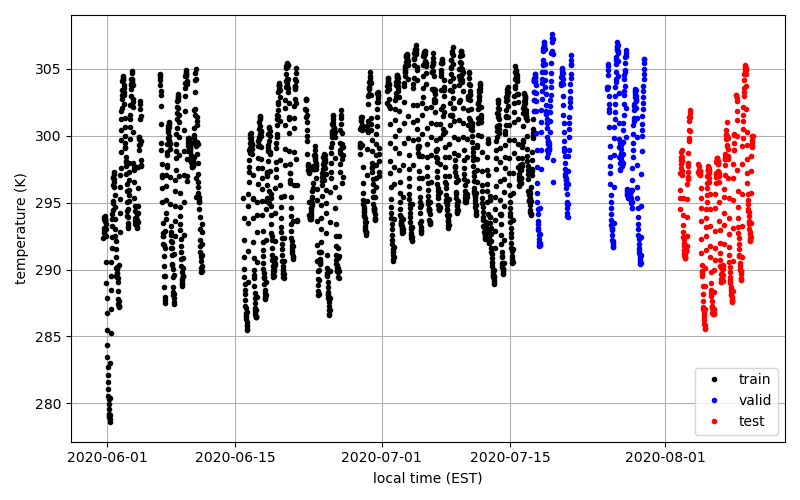
\includegraphics[width=0.49\textwidth]{temporal_sequence_temp.png}
	}
	\subfloat[Pressure (Pa)\label{fig:sequence_temporal_b}]{
		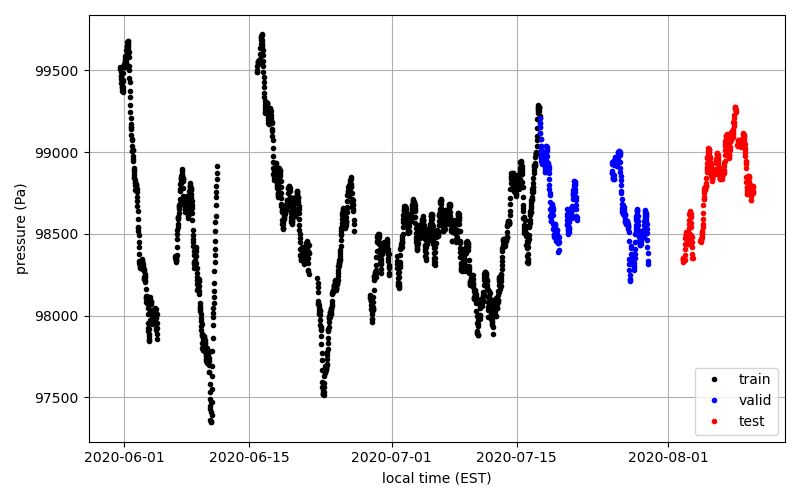
\includegraphics[width=0.49\textwidth]{temporal_sequence_press.png}
	}
	\hfill
	\subfloat[Relative Humidity (\%)\label{fig:sequence_temporal_c}]{
		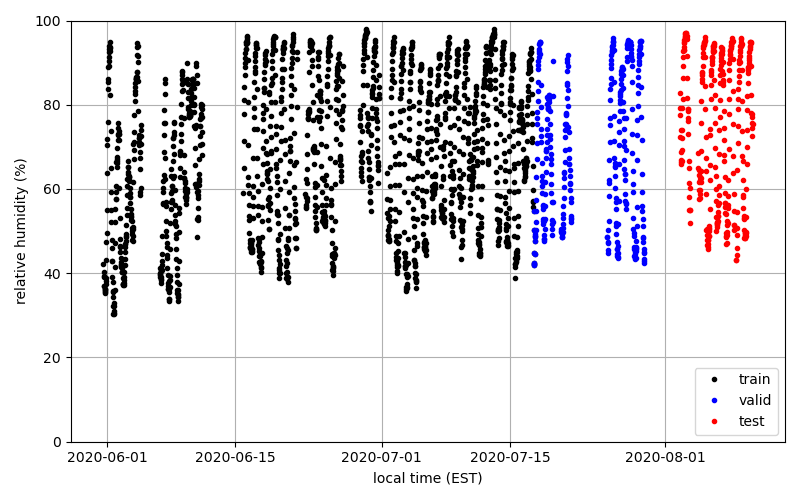
\includegraphics[width=0.49\textwidth]{temporal_sequence_rh.png}
	}
	\subfloat[Wind Speed (m/s)\label{fig:sequence_temporal_d}]{
		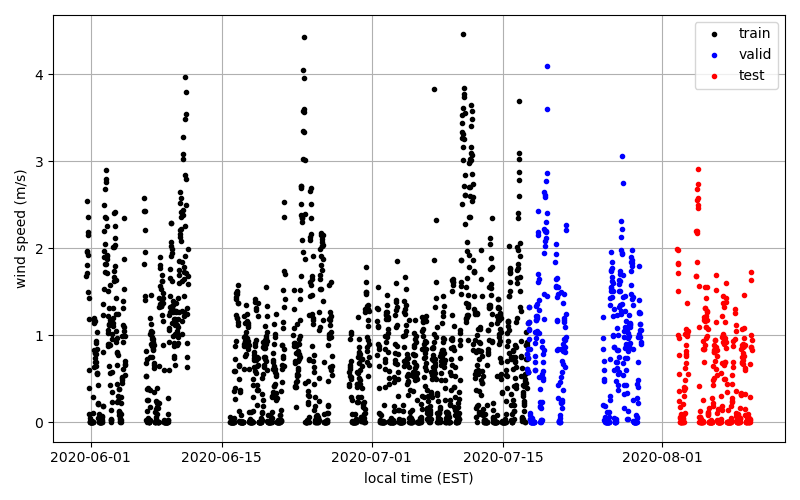
\includegraphics[width=0.49\textwidth]{temporal_sequence_wind_spd.png}
	}
	\hfill
	\subfloat[Solar Irradiance ($W/m^{2}$)\label{fig:sequence_temporal_e}]{
		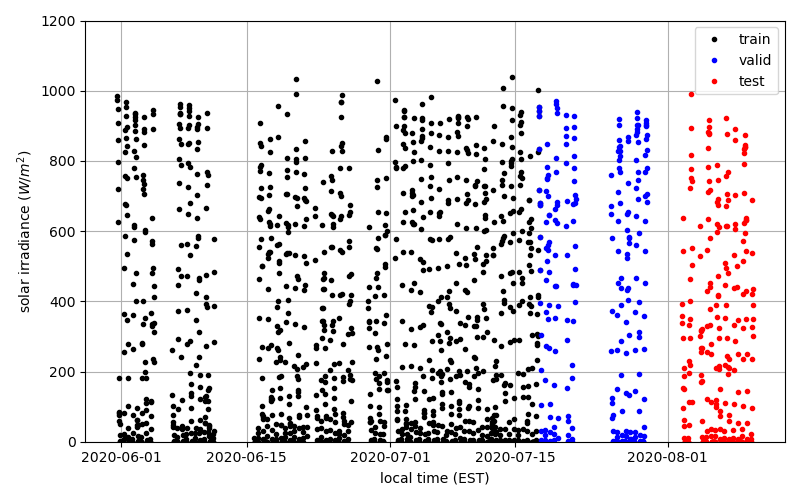
\includegraphics[width=0.49\textwidth]{temporal_sequence_solar_irr.png}
	}
	\subfloat[Turbulence $C_{n}^{2}$ ($m^{-2/3}$)\label{fig:sequence_temporal_f}]{
		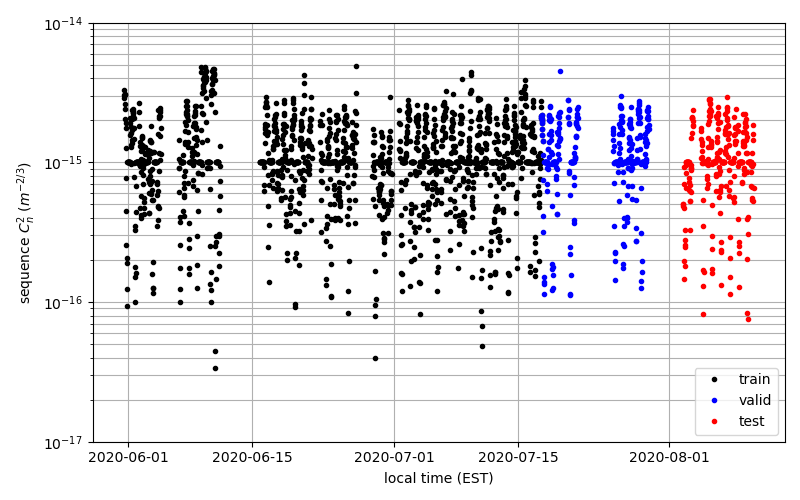
\includegraphics[width=0.49\textwidth]{temporal_sequence_cn2.png}
	}
	\hfill
	\caption{Sequence data as a function of time, parsed by train, validation, and test datasets drawn in black, blue, and red, respectively.}
	\label{fig:sequence_temporal}
\end{figure}
Temperature, pressure, relative humidity, wind speed, solar irradiance, and nighttime-filled $C_{n}^{2}$ are in Figures \ref{fig:sequence_temporal_a} - \ref{fig:sequence_temporal_f}, respectively. The plotted measurements are after the data processing described above, so they're at 30-minute intervals after filtering, window averaging and interpolating. Furthermore in each plot, the train, validation, and test datasets are plotted with black, blue, and red markers, respectively. The train dataset spans from 01 June through 17 July. The validation dataset spans from 18 July through 01 August. Finally, the test dataset spans from 02 - 10 August. Of the 1255 sequence/forecast pairs, 933 (74.3\%) are in the train dataset, 174 (13.9\%) in the validation dataset, and 148 (11.8\%) in the test dataset.

The measurements in Figure \ref{fig:sequence_temporal} illustrate many interesting features. First for temperature in Figure \ref{fig:sequence_temporal_a}, the positive result of only using data from June through August is shown. Across the entire dataset, except for the very first day, the temperature measurements are within about 20 Kelvin. Further, the validation dataset (blue) is a great representation of the train dataset (black). The test dataset (red) has a few cold days in the beginning, but then warms up again. This cold snap is not ideal, but is well within the dynamic range of the train and validation datasets. Pressure in Figure \ref{fig:sequence_temporal_b} shows that long, large scale measurements are made in June but in July and August the measurements are on a shorter scale. The validation and test pressure datasets are well within the dynamic range of the train dataset, but do not illustrate clearly similar trends.

Relative humidity in Figure \ref{fig:sequence_temporal_c} is a very stable weather measurement across the train, validation, and test datasets. The measurements never drop below 30\%, and the validation and test datasets are within the dynamic range of the train dataset. The oscillatory nature of relative humidity is shown in Figure \ref{fig:sequence_temporal_c} and appears consistent between the three datasets. Wind speed in Figure \ref{fig:sequence_temporal_d} is not a stable measurement. An oscillatory nature is not apparent, and wind speed is a significant driver of weather events as shown by the spikes in measurements, especially in the train dataset. Commonality between the three datasets in Figure \ref{fig:sequence_temporal_d} are not clearly extracted.

Solar irradiance in Figure \ref{fig:sequence_temporal_e} is another stable weather measurement across the three datasets. The model is expected to learn the temporal aspect of solar irradiance, i.e., a measurement of 0 (zero) indicates nighttime, and also the variation from a standard diurnal trend is due to cloud conditions which is typically associated with $C_{n}^{2}$ conditions which also deviate from a standard diurnal trend. Solar irradiance is directly impacted by the seasonal weather change (Earth's axial tilt). The highest solar irradiance measurements for a day are in summertime, specifically around the summer solstice. The highest measurement of the day gradually decreases from the summer solstice to a minimum around the winter solstice. This effect is not clearly shown in Figure \ref{fig:sequence_temporal_e} since only summertime is considered.

Sequence $C_{n}^{2}$ in Figure \ref{fig:sequence_temporal_f} illustrates stability and the impact of nighttime filling with $1 \times 10^{-15} (m^{-2/3})$. First, the test and validation datasets are strongly representative of the train dataset. Besides a few instances in the whole dataset, the maximum $C_{n}^{2}$ does not increase above $3 \times 10^{-15} (m^{-2/3})$. Daily oscillation of $C_{n}^{2}$ is apparent in Figure \ref{fig:sequence_temporal_f} and is the standard diurnal trend. The low-strength $C_{n}^{2}$ conditions are much more variable than high-strength conditions. There are several examples of $C_{n}^{2}$ weather than $1 \times 10^{-16} (m^{-2/3})$ but they are spread through the entire dataset. These events are associated with particularly strong evening neutral events. The line of markers at $1 \times 10^{-15} (m^{-2/3})$ in Figure \ref{fig:sequence_temporal_f} is the nighttime padding. These padded measurements are strongly correlated with the $0 W/m^{2}$ solar irradiance measurements in Figure \ref{fig:sequence_temporal_e}.

The relationship of the train, validation, and test datasets is further shown in Figure \ref{fig:sequence_histograms} which plots probability densities of each input sequence variable. Temperature, pressure, relative humidity, wind speed, solar irradiance, and nighttime filled $C_{n}^{2}$ are plotted in Figures \ref{fig:sequence_histograms_a} through \ref{fig:sequence_histograms_f}, respectively. Similarly to the temporal plots, the black bars in Figure \ref{fig:sequence_histograms} represent the train dataset, blue bars the validation dataset, and red bars the test dataset.
\begin{figure}[p!]
	\centering
	\subfloat[Temperature (K)\label{fig:sequence_histograms_a}]{
		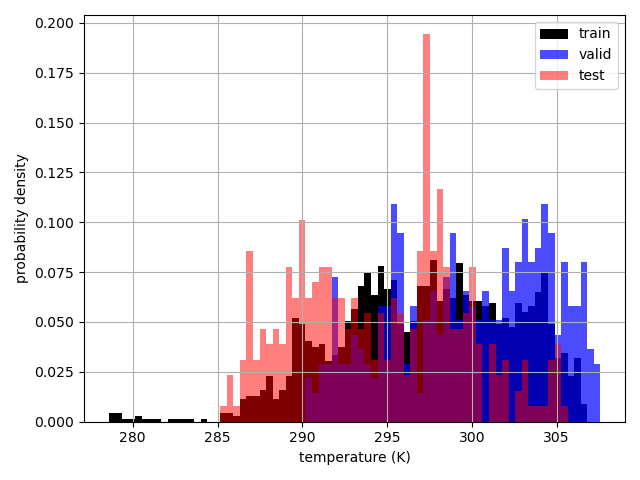
\includegraphics[width=0.49\textwidth]{hist_sequence_temp.png}
	}
	\subfloat[Pressure (Pa)\label{fig:sequence_histograms_b}]{
		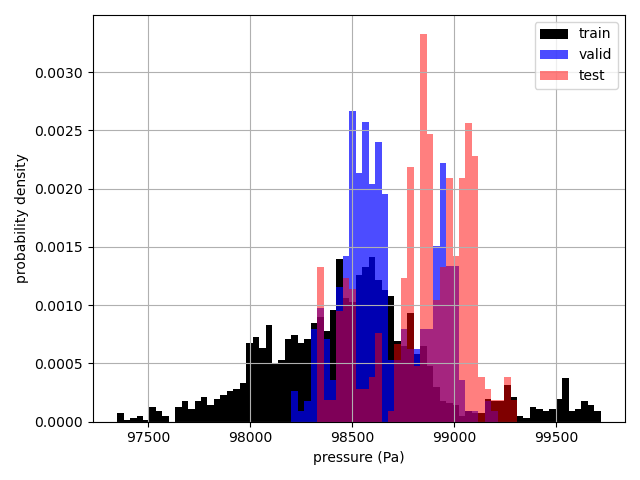
\includegraphics[width=0.49\textwidth]{hist_sequence_press.png}
	}
	\hfill
	\subfloat[Relative Humidity (\%)\label{fig:sequence_histograms_c}]{
		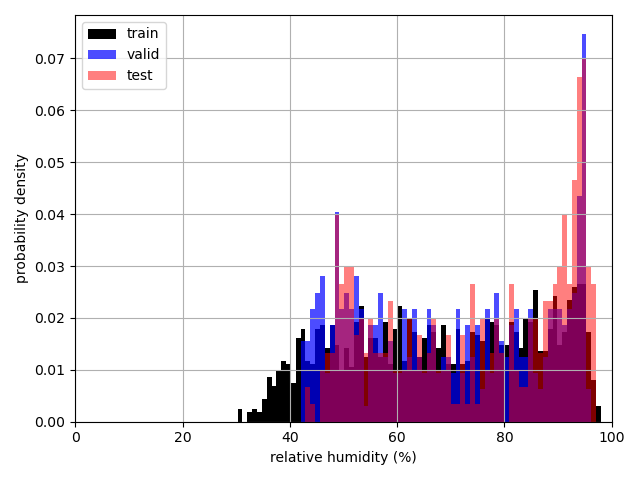
\includegraphics[width=0.49\textwidth]{hist_sequence_rh.png}
	}
	\subfloat[Wind Speed (m/s)\label{fig:sequence_histograms_d}]{
		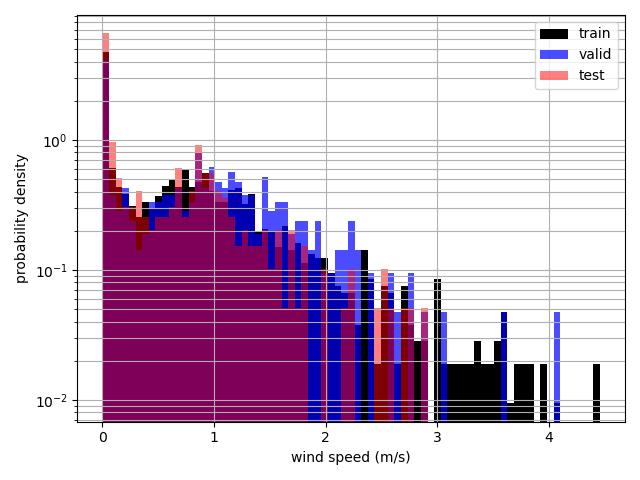
\includegraphics[width=0.49\textwidth]{hist_sequence_wind_spd.png}
	}
	\hfill
	\subfloat[Solar Irradiance\label{fig:sequence_histograms_e}]{
		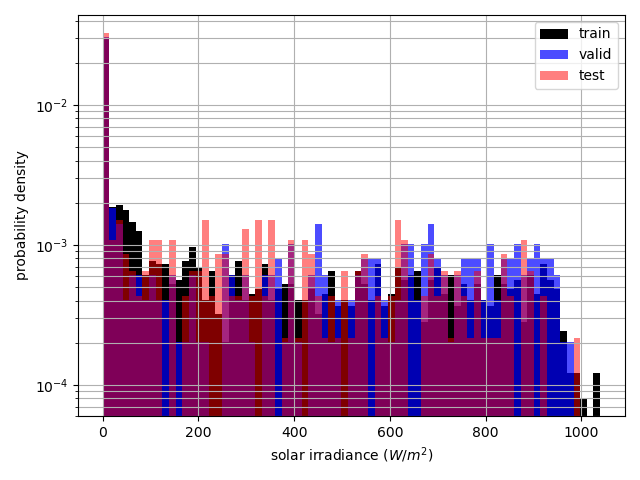
\includegraphics[width=0.49\textwidth]{hist_sequence_solar_irr.png}
	}
	\subfloat[Nighttime-filled $log_{10}(C_{n}^{2}$)\label{fig:sequence_histograms_f}]{
		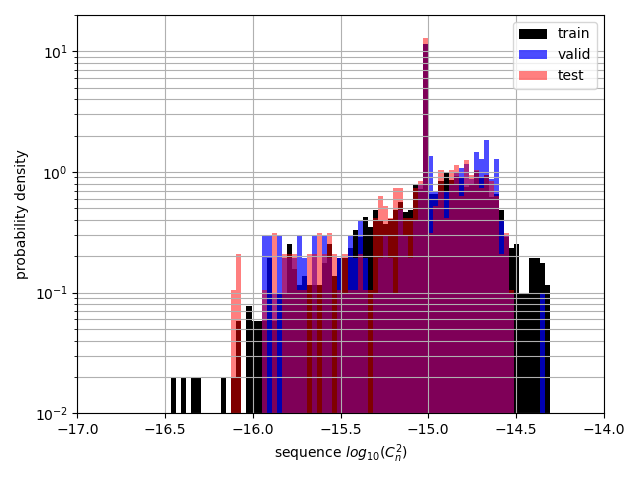
\includegraphics[width=0.49\textwidth]{hist_sequence_cn2.png}
	}
	\hfill
	\caption{Sequence data in normalized histograms, parsed by the train, validation, and test datasets drawn in black, blue, and red, respectively.}
	\label{fig:sequence_histograms}
\end{figure}
The bars in each plot of Figure \ref{fig:sequence_histograms} represent how the \emph{distribution} of the three datasets relate to each other. They also explicitly show how the dynamic range of the validation and test datasets relate to the dynamic range of the train dataset.

Temperature in Figure \ref{fig:sequence_histograms_a} shows that the distribution of the validation dataset is near the high-temperature portion of the train dataset since the blue bars are to the right of the plot. There are even blue bars at the very high temperatures where there are no black bars which is indicative that there are measurements in the validation dataset which are hotter than anything in the train dataset. This is an example where the model is forced to extrapolate given input measurements its never encountered in training. The test dataset (red bars) is at the lower end (left side) of the temperature distributions indicative that colder temperatures are part of the test measurements. These low temperature measurements are still within the bounds of the train dataset dynamic range since there are black bars to the far left of Figure \ref{fig:sequence_histograms_a}. The features of these distributions are consistent with the features noted in the temporal plot in Figure \ref{fig:sequence_temporal_a}.

Pressure in Figure \ref{fig:sequence_histograms_b} shows that the temperature distribution is most populated around 98,500 Pa and looks similar to a Gaussian distribution. The validation dataset is mostly distributed around the center of the train distribution, an encouraging feature. The test dataset is similarly distributed but a scale factor higher around 99,000 Pa. There is also a significant amount of validation dataset pressure measurements around this value.

Relative humidity in Figure \ref{fig:sequence_histograms_c} illustrates the stability between the three datasets first described above. The distribution of the three bar sets are very similar in shape and magnitude. The spike in probability just below 100\% and the slight rise around 50\% is characteristic of all three datasets. The distribution between is likewise very similar. Figure \ref{fig:sequence_histograms_c} illustrates an ideal case for the datasets to be highly representative of each other.

Wind speed in Figure \ref{fig:sequence_histograms_d} is the first histogram to show comparison that is more encouraging than the temporal plots in Figure \ref{fig:sequence_temporal}. The shape of the three distributions in Figure \ref{fig:sequence_histograms_d} are very similar from wind speeds of 0 m/s to about 2 m/s. The spike in measurements at 0 m/s is highly consistent among the three distributions. The sharp drop off back to another increase around 1 m/s, and the gradual decline in probability from 1 m/s to 2 m/s is also consistent. The validation distribution continues to follow the train distribution beyond 2 m/s, but the test measurements become far more sparse. Figure \ref{fig:sequence_histograms_d} indicates that below 2 m/s the validation and test distributions are highly representative of each other. However, the temporal trends of wind speed are most relevant to this problem and that is not illustrated in the histogram. As stated earlier, the temporal trends in wind speed  are not clear in Figure \ref{fig:sequence_temporal_d}. The validation distribution is within the train distribution, and the test distribution even more so.

The solar irradiance distributions in Figure \ref{fig:sequence_histograms_e} are highly representative of each other. The spike in probability density at $0 W/m^{2}$ is nearly identical across the three distributions. Furthermore, the shape of the distributions up to $1000 W/m^{2}$ are also very similar. Some gaps exist in the test dataset, but the general distribution is representative. Most importantly, the validation and test distributions are within the dynamic range of the train distribution.

Finally, nighttime-filled $log_{10}(C_{n}^{2})$ in Figure \ref{fig:sequence_histograms_f} again illustrates very similar distributions between the three datasets. For the majority of the measurements from about -15.75 through -14.5 the distributions are nearly identical. The spike in probability at -15 is due to the nighttime filling. The dynamic range of the validation and test datasets are mostly well within the bounds of the train dataset. Generally, the relationship of the distributions in Figure \ref{fig:sequence_histograms_f} is an ideal scenario.

The other part of the sequence/forecast pair is the forecasts. Figure \ref{fig:forecast_sequence_histogram} illustrates the temporal and histogram plots in Figures \ref{fig:forecast_sequence_histogram_a} and \ref{fig:forecast_sequence_histogram_b}. These plots are nearly identical to input sequence $C_{n}^{2}$ Figures \ref{fig:sequence_temporal_f} and \ref{fig:sequence_histograms_f} with the primary difference being the lack of nighttime measurement filling at $1 \times 10^{-15} (m^{-2/3})$.
\begin{figure}[h!]
	\centering
	\subfloat[\label{fig:forecast_sequence_histogram_a}]{
		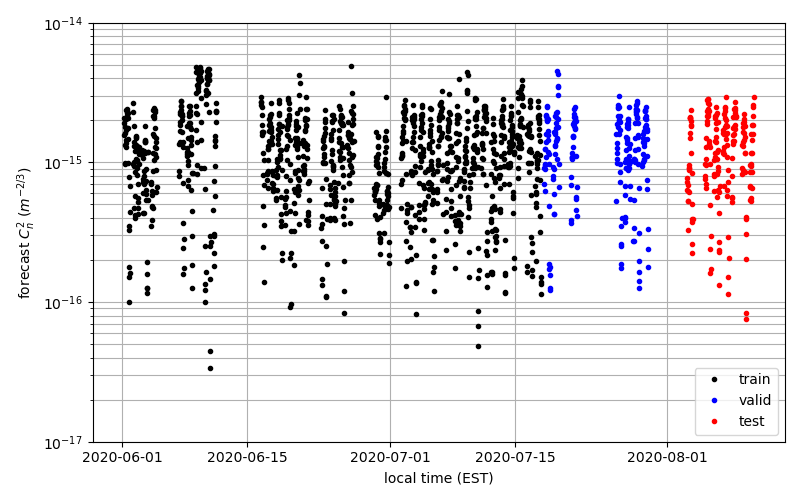
\includegraphics[width=0.543\textwidth]{temporal_forecast_cn2.png}
	}
	\subfloat[\label{fig:forecast_sequence_histogram_b}]{
		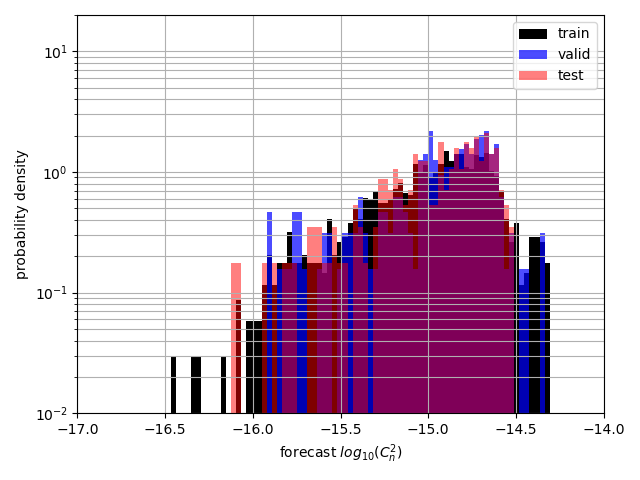
\includegraphics[width=0.447\textwidth]{hist_forecast_cn2.png}
	}
	\hfill
	\caption{Turbulence ($C_{n}^{2}$) forecasts as a function of time and as a normalized histogram. The train, validation, and test datasets are drawn in black, blue, and red, respectively.}
	\label{fig:forecast_sequence_histogram}
\end{figure}
This is shown as the missing line of markers in Figure \ref{fig:forecast_sequence_histogram_a} and the missing spike in Figure \ref{fig:forecast_sequence_histogram_b}. The three datasets are very similar both temporally and in their distributions, again a highly desirable quality.  An interesting feature about the three datasets in Figure \ref{fig:forecast_sequence_histogram_a} is that the validation dataset has a measurement above $3 \times 10^{-15} (m^{-2/3})$ but the test dataset does not. Furthermore the validation dataset does not have any measurements weaker than $1 \times 10^{-16} (m^{-2/3})$ but the test dataset has two. The histogram in Figure \ref{fig:forecast_sequence_histogram_b} reflects this. These features are the most significant difference between the three datasets and potentially could impact the parameter selection process and final model evaluation. The parameter selection process is evaluated on a dataset which does not have any extremely deep $C_{n}^{2}$ events. Therefore the best model could be a model which does not learn to handle these deep neutral events at all which will result in poor performance on the deep neutral event in the test dataset. Furthermore, the validation dataset has an event of abnormally strong $C_{n}^{2}$. This could also lead the best model to handle these events well but will not be reflected in the final model evaluation since an event of this sort is not in the test dataset.

Overall, the sequences and forecasts presented in Figures \ref{fig:sequence_temporal}, \ref{fig:sequence_histograms}, and \ref{fig:forecast_sequence_histogram} show that the train, validation, and test datasets are strong representations of each other, and there are no significant changes in weather patterns on a day-to-day and seasonal basis. Also, a few measurements of temperature is the only instance of a validation or test measurement being beyond the dynamic range of the train dataset. This small outlier does not propagate to the test dataset because the final model is trained on the combination of train and validation datasets. These are highly desirable characteristics for a machine learning study.

%\begin{figure}[h!]
%	\centering
%	\includegraphics[width=0.99\textwidth]
%	{example_sequence_forecast.png}
%	\hfill
%	\caption{Example sequence and corresponding turbulence forecast. \textbf{NEED TO ADD WIND SPEED AND PRIOR TURBULENCE MEASUREMENTS}}
%	\label{fig:example_sequence_forecast}
%\end{figure}

\subsubsection{Data Normalization}
With the sequence/forecast pairs for training, validation, and testing, the final step in data processing is to normalize the data for training and inference. The normalization parameters are derived from the train dataset, but are applied to the train, validation, and test datasets. In this work each input variable and output $C_{n}^{2}$ from the train dataset are min-max ranged between 0 and 1 using
\begin{equation} \label{eq:normalize_data}
	\hat{x} = \frac{x - x_{min}}{x_{max} - x_{min}},
\end{equation}
where $x$ is the variable considered, $x_{min}$ is the minimum of $x$, $x_{max}$ is the maximum of $x$, and $\hat{x}$ is the normalized variable. To ensure stability, data normalization for $C_{n}^{2}$ is applied to the $log_{10}(C_{n}^{2})$ since values associated with turbulence are most often smaller than $1 \times 10^{-12} (m^{-2/3})$. The normalization parameters $x_{max}$ and $x_{min}$ are saved then Equation \ref{eq:normalize_data} is applied to the validation and test datasets. Any measurements outside of $x_{max}$ or $x_{min}$ will normalize to beyond 0 and 1.

Throughout this work evaluation of model performance is done in $log_{10}(C_{n}^{2})$ space so model outputs must be unnormalized by
\begin{equation} \label{eq:unnormalize_data}
	x = \hat{x} \cdot \left(x_{max} - x_{min}\right) + x_{min}
\end{equation}
and compared with the unnormalized measurement $C_{n}^{2}$ forecasts.

\section{Chapter Summary?}